% Version 3.5 March 2018
%
% % % % % % % % % % % % % % % % % % % % % %
%
% -- IMPORTANT NOTE
%
% This template contains comments intended 
% to minimize problems and delays during our production 
% process. Please follow the template instructions
% whenever possible.
%
% % % % % % % % % % % % % % % % % % % % % % % 
%
% Once your paper is accepted for publication, 
% PLEASE REMOVE ALL TRACKED CHANGES in this file 
% and leave only the final text of your manuscript. 
% PLOS recommends the use of latexdiff to track changes during review, as this will help to maintain a clean tex file.
% Visit https://www.ctan.org/pkg/latexdiff?lang=en for info or contact us at latex@plos.org.
%
%
% There are no restrictions on package use within the LaTeX files except that 
% no packages listed in the template may be deleted.
%
% Please do not include colors or graphics in the text.
%
% The manuscript LaTeX source should be contained within a single file (do not use \input, \externaldocument, or similar commands).
%
% % % % % % % % % % % % % % % % % % % % % % %
%
% -- FIGURES AND TABLES
%
% Please include tables/figure captions directly after the paragraph where they are first cited in the text.
%
% DO NOT INCLUDE GRAPHICS IN YOUR MANUSCRIPT
% - Figures should be uploaded separately from your manuscript file. 
% - Figures generated using LaTeX should be extracted and removed from the PDF before submission. 
% - Figures containing multiple panels/subfigures must be combined into one image file before submission.
% For figure citations, please use "Fig" instead of "Figure".
% See http://journals.plos.org/plosone/s/figures for PLOS figure guidelines.
%
% Tables should be cell-based and may not contain:
% - spacing/line breaks within cells to alter layout or alignment
% - do not nest tabular environments (no tabular environments within tabular environments)
% - no graphics or colored text (cell background color/shading OK)
% See http://journals.plos.org/plosone/s/tables for table guidelines.
%
% For tables that exceed the width of the text column, use the adjustwidth environment as illustrated in the example table in text below.
%
% % % % % % % % % % % % % % % % % % % % % % % %
%
% -- EQUATIONS, MATH SYMBOLS, SUBSCRIPTS, AND SUPERSCRIPTS
%
% IMPORTANT
% Below are a few tips to help format your equations and other special characters according to our specifications. For more tips to help reduce the possibility of formatting errors during conversion, please see our LaTeX guidelines at http://journals.plos.org/plosone/s/latex
%
% For inline equations, please be sure to include all portions of an equation in the math environment.  For example, x$^2$ is incorrect; this should be formatted as $x^2$ (or $\mathrm{x}^2$ if the romanized font is desired).
%
% Do not include text that is not math in the math environment. For example, CO2 should be written as CO\textsubscript{2} instead of CO$_2$.
%
% Please add line breaks to long display equations when possible in order to fit size of the column. 
%
% For inline equations, please do not include punctuation (commas, etc) within the math environment unless this is part of the equation.
%
% When adding superscript or subscripts outside of brackets/braces, please group using {}.  For example, change "[U(D,E,\gamma)]^2" to "{[U(D,E,\gamma)]}^2". 
%
% Do not use \cal for caligraphic font.  Instead, use \mathcal{}
%
% % % % % % % % % % % % % % % % % % % % % % % % 
%
% Please contact latex@plos.org with any questions.
%
% % % % % % % % % % % % % % % % % % % % % % % %

\documentclass[10pt,letterpaper]{article}
\usepackage[top=0.85in,left=2.75in,footskip=0.75in]{geometry}

% TODO remove before submission
\usepackage{setspace}
\doublespacing

% amsmath and amssymb packages, useful for mathematical formulas and symbols
\usepackage{amsmath,amssymb}

% Use adjustwidth environment to exceed column width (see example table in text)
\usepackage{changepage}

% Use Unicode characters when possible
\usepackage[utf8x]{inputenc}

% textcomp package and marvosym package for additional characters
\usepackage{textcomp,marvosym}

% cite package, to clean up citations in the main text. Do not remove.
\usepackage{cite}

\usepackage{listings}

\usepackage{csquotes}

% Use nameref to cite supporting information files (see Supporting Information section for more info)
\usepackage{nameref,hyperref}
\hypersetup{
    colorlinks=true,
    linkcolor=blue,
    filecolor=magenta,      
    urlcolor=cyan,
}

% line numbers
\usepackage[right]{lineno}

% ligatures disabled
\usepackage{microtype}
\DisableLigatures[f]{encoding = *, family = * }

% color can be used to apply background shading to table cells only
\usepackage[table]{xcolor}

% array package and thick rules for tables
\usepackage{array}

% create "+" rule type for thick vertical lines
\newcolumntype{+}{!{\vrule width 2pt}}

% create \thickcline for thick horizontal lines of variable length
\newlength\savedwidth
\newcommand\thickcline[1]{%
  \noalign{\global\savedwidth\arrayrulewidth\global\arrayrulewidth 2pt}%
  \cline{#1}%
  \noalign{\vskip\arrayrulewidth}%
  \noalign{\global\arrayrulewidth\savedwidth}%
}

% \thickhline command for thick horizontal lines that span the table
\newcommand\thickhline{\noalign{\global\savedwidth\arrayrulewidth\global\arrayrulewidth 2pt}%
\hline
\noalign{\global\arrayrulewidth\savedwidth}}


% Remove comment for double spacing
%\usepackage{setspace} 
%\doublespacing

% Text layout
\raggedright
\setlength{\parindent}{0.5cm}
\textwidth 5.25in 
\textheight 8.75in

% Bold the 'Figure #' in the caption and separate it from the title/caption with a period
% Captions will be left justified
\usepackage[aboveskip=1pt,labelfont=bf,labelsep=period,justification=raggedright,singlelinecheck=off]{caption}
\renewcommand{\figurename}{Fig}

\usepackage{textgreek}


% Use the PLoS provided BiBTeX style
\bibliographystyle{plos2015}

% Remove brackets from numbering in List of References
\makeatletter
\renewcommand{\@biblabel}[1]{\quad#1.}
\makeatother



% Header and Footer with logo
\usepackage{lastpage,fancyhdr,graphicx}
\usepackage{epstopdf}
%\pagestyle{myheadings}
\pagestyle{fancy}
\fancyhf{}
%\setlength{\headheight}{27.023pt}
%\lhead{\includegraphics[width=2.0in]{PLOS-submission.eps}}
\rfoot{\thepage/\pageref{LastPage}}
\renewcommand{\headrulewidth}{0pt}
\renewcommand{\footrule}{\hrule height 2pt \vspace{2mm}}
\fancyheadoffset[L]{2.25in}
\fancyfootoffset[L]{2.25in}
\lfoot{\today}

%% Include all macros below

\newcommand{\lorem}{{\bf LOREM}}
\newcommand{\ipsum}{{\bf IPSUM}}

%% END MACROS SECTION


\begin{document}
\vspace*{0.2in}

% Title must be 250 characters or less.
\begin{flushleft}
{\Large
\textbf\newline{Towards development of statistical techniques to evaluate myotonic dystrophy type 1 mRNA biomarkers in the context of a clinical trial} % Please use "sentence case" for title and headings (capitalize only the first word in a title (or heading), the first word in a subtitle (or subheading), and any proper nouns).
}
\newline
% Insert author names, affiliations and corresponding author email (do not include titles, positions, or degrees).
\\
Adam Kurkiewicz\textsuperscript{1},
Anneli Cooper\textsuperscript{3}{\textcurrency},
Guillaume Bassez\textsuperscript{4},
Bruno Eymard\textsuperscript{5},
Ralf Krahe\textsuperscript{6},
Mani Mahadevan\textsuperscript{7},
Giovanni Meola\textsuperscript{8},
Jack Puymirat\textsuperscript{9},
Mark Rogers\textsuperscript{10},
Benedikt Schoser\textsuperscript{11},
Lubov Timchenko\textsuperscript{12},
Baziel van Engelen\textsuperscript{13},
Tetsuo Ashizawa \textsuperscript{14},
Richard Moxley \textsuperscript{15},
Simon Rogers\textsuperscript{2}{\Yinyang},
John McClure\textsuperscript{1}{\Yinyang},
Darren G Monckton\textsuperscript{3*}{\Yinyang},
with Dystrophia Myotonica Biomarker Discovery Initative
\\
\bigskip
\textbf{1} Institute of Cardiovascular and Medical Sciences, University of Glasgow, Glasgow, United Kingdom
\\
\textbf{2} School of Computing Science, University of Glasgow, Glasgow, United Kingdom
\\
\textbf{3} Institute of Molecular Cell and Systems Biology, University of Glasgow, Glasgow, United Kingdom
\\
\textbf{4} Département de Pathologie, CHU Henri Mondor, Créteil Cedex, France
\\
\textbf{5} Neuromuscular Pathology Clinical Unit, Myology Institute, Salpêtrière Hospital, Paris, France
\\
\textbf{6} Dept of Cancer Genetics, MD Anderson Cancer Center, University of Texas, Houston, TX, USA
\\
\textbf{7} Department of Pathology, Molecular Diagnostics Lab, University of Virginia, Charlottesville, VA, USA
\\
\textbf{8} Department of Neurology, IRCCS Policlinico Sandonato, Milan, Italy
\\
\textbf{9} Laboratory of Human Genetics, CHUL Medical Research Centre, University of Laval, Quebec City, QC, Canada
\\
\textbf{10} University Hospital of Wales, Cardiff, Wales
\\
\textbf{11} Friedrich Baur Institute, Department of Neurology, Ludwig Maximilians University, Munich, Germany
\\
\textbf{12} Department of Molecular Physiology and Biophysics, Baylor College of Medicine, Houston, TX, USA
\\
\textbf{13} Neuromuscular Centre Nijmegen, Department of Neurology, Radboud University Medical Centre, Nijmegen, The Netherlands
\\
\textbf{14} VA Medical Center, Houston, Texas, USA
\\
\textbf{15} University of Rochester, Medical Center
School of Medicine and Dentistry, Rochester, New York, USA
\bigskip

% Insert additional author notes using the symbols described below. Insert symbol callouts after author names as necessary.
% 
% Remove or comment out the author notes below if they aren't used.
%
% Primary Equal Contribution Note
\Yinyang These authors contributed equally to this work.

% Additional Equal Contribution Note
% Also use this double-dagger symbol for special authorship notes, such as senior authorship.
% \ddag These authors also contributed equally to this work.

% Current address notes
\textcurrency Institute of Biodiversity, Animal Health and Comparative Medicine, University of Glasgow, Glasgow, United Kingdom % change symbol to "\textcurrency a" if more than one current address note
% \textcurrency b Insert second current address 
% \textcurrency c Insert third current address

% Deceased author note
% \dag Deceased

% Group/Consortium Author Note
% \textpilcrow Membership list can be found in the Acknowledgments section.

% Use the asterisk to denote corresponding authorship and provide email address in note below.
* darren.monckton@glasgow.ac.uk

\end{flushleft}
% Please keep the abstract below 300 words
\section*{Abstract}

Myotonic dystrophy type 1 (DM1) is a rare genetic disorder, characterised by anticipation of muscular dystrophy, myotonia, and other symptoms. DM1 is caused by the expansion of a CTG repeat in the 3' untranslated region of {\it DMPK}. Longer CTG expansions are associated with greater symptom severity and earlier age at onset. The primary mechanism of pathogenesis is thought to be mediated by a gain of function of the CUG-containing RNA, that leads to {\it trans}-dysregulation of RNA metabolism of many other genes. Specifically, the alternative splicing (AS) and alternative polyadenylation (APA) of many genes is known to be disrupted. In a context of a clinical trial of emerging DM1 treatments, it is important to be able to objectively quantify treatment efficacy at the level of molecular biomarkers. We show how previously described candidate mRNA biomarkers, can be used to model an {\it effective} reduction in CTG length, using modern high-dimensional statistcs (machine learning), and a previously unpublished blood an muscle mRNA microarray dataset. We show how this model can be used to detect treatment effect in the context of a clinical trial.

% Please keep the Author Summary between 150 and 200 words
% Use first person. PLOS ONE authors please skip this step. 
% Author Summary not valid for PLOS ONE submissions.   
% \section*{Author summary}
% Lorem ipsum dolor sit amet, consectetur adipiscing elit. Curabitur eget porta erat. Morbi consectetur est vel gravida pretium. Suspendisse ut dui eu ante cursus gravida non sed sem. Nullam sapien tellus, commodo id velit id, eleifend volutpat quam. Phasellus mauris velit, dapibus finibus elementum vel, pulvinar non tellus. Nunc pellentesque pretium diam, quis maximus dolor faucibus id. Nunc convallis sodales ante, ut ullamcorper est egestas vitae. Nam sit amet enim ultrices, ultrices elit pulvinar, volutpat risus.

\linenumbers

% Use "Eq" instead of "Equation" for equation citations.
\section*{Introduction}

\subsection*{Myotonic dystrophy type 1}

Myotonic dystrophy type 1 (DM1) is an autosomal dominant trinucleotide repeat disorder, caused by abnormally large CTG repeat in a 3' UTR of the gene encoding {\it dystrophia myotonica protein kinase} ({\it DMPK}) \cite{Brook1992}. Transcription of {\it DMPK} in affected individuals produces a toxic, GC-rich mRNA molecule, which dysregulates several RNA binding factors, including proteins MBNL1, MBNL2, MBNL3, CUGBP1, hnRNP H and Staufen1 \cite{Meola2015}. The pathomechanism of the dysregulation of a splicing factor MBNL1 is perhaps best understood, with MBNL1 sequestration to the toxic {\it DMPK} RNA product resulting in splicing defects of pre-mRNAs of multiple genes, including chloride channel ({\it CLCN1}), brain microtubule-associated
tau ({\it MAPT}) and insulin receptor ({\it INSR}) \cite{Holt2009}. Such splicing defects are direct cause or major contributing factor of clinical symptomps of DM1, such as myotonia ({\it CLCN1}), abnormal glucose response ({\it INSR}), cardiac conduction defects ({\it TNNT2}), and are hypothesised to play a role in other clinical symptoms, including muscle wasting, cataracts, hypersomnia, gastrointestinal abnormalities, as well as premature baldness and testicular atrophy in males \cite{Meola2015} \cite{Udd2012}. The severity of symptoms is positively correlated with CTG repeat length \cite{Meola2015}.

Toxic {\it DMPK} transcript in DM1-affected individuals was identified as an active target for theraupetic intervation \cite{Pandey2015}, and it is expected that breakdown or deactivation of the toxic mRNA will result in at least partial reversal of DM1-induced AS changes and other known and unknown DM1-induced biomolecular pathologies.

Spliceopathy of DM1 is an active area of research, with novel splicing defects being continuously reported. Nakamori {\it et al.} \cite{Nakamori2013} identified a set of 41 genes, which are mis-spliced in DM1, suggesting these genes as potential biomarkers of DM1. Batra {\it et al.} \cite{Batra2014} identified 80 genes, whose expression indicates disrupted APA, reusing the (human) dataset of Nakamori {\it et al.} and using other datasets, including data from mouse models.

\subsection*{Predictors in genetics research}

A widespread paradigm in biological and clinical research are case-control studies, using frequentist statistics tools focusing on hypothesis testing (inference). Examples of such tools include GWAS designs \cite{Bush2012}, placebo and active control clinical trial designs \cite{Brody2016}, non-inferiority designs \cite{DAgostino2002} or heredity designs based on twin studies. It is reported that designs of as many as 70\%  of studies published in leading medical journals use at most the following three statistical tests as part of their design: Student's t-test, Fisher's exact test and Chi-square test \cite{Prel2010}.

A possible alternative to the focus on hypothesis testing is building predictors or classifiers, which produce a numerical estimate of a given trait (height, size of the DM1 trinucleotide expansion) or effect size, predict participant's category (such as affected/unaffected) or estimate the effect size of the treatment, given a set of independent variables (e.g. genotypes, mRNA profiles, etc.). If necessary, the efficacy of these predictors/classifiers can be evaluated using traditional frequentist tools, such as p-values.

Predictors have been successfully applied in genetics research. For example, Lello {\it et al.} \cite{Lello2017} report predicting human height from genotype data, obtained using human SNP microarrays, to within a few centimeters for most participants in their sample. This level of accuracy is achieved by a very large sample size of nearly half a million individuals. A review by Van Raden {\it et al.} \cite{VanRaden2009} reports ability to predict dairy output of certain cattle breeds with R\textsuperscript{2} of 49\%, using non-linear models based on SNP microarrays. The work of Azencott {\it et al.} \cite{Azencott2013} allows to incorporate prior information about biological networks into the predictive model, increasing prediction accuracy, and again is targeting the genomics community. In a work, which is one of direct motivations behind our research, Lee {\it et al.} \cite{Lee2013} report being able to predict most of Huntington disease trinucleotide repeat size using mRNA profiling of lymphoblastoid cell lines. In this paper we demonstrate a further application of predictors in genetics research, by constructing a predictor, which can produce a numerical estimate of a participant's DM1 CTG repeat from an mRNA profile, and demonstrate its usefulness in the context of a hypothetical clinical trial of a DM1 treatment.

\subsection*{Prior identification of alternative splicing and alternative polyadenylation events in muscles of DM1-affected individuals}\label{prior_work}

Our primary reference is the work of Nakamori {\it et al.} \cite{Nakamori2013}, who identified 42 genes exhibiting AS defects in DM1. Briefly, their methodology was as follows:
Muscle tissue (patients: four biceps, two quadriceps, one tibialis anterior, one diaphragm; controls: eight vastus lateralis) were sampled post-mortem from eight DM1 affected participants and eight unaffected controls.
mRNA was extracted from the samples, purified and hybridized to GeneChip™ Human Exon 1.0 ST microarrays.
Putative AS defects were identified using a mixture of existing methods, such as Affymetrix's PLIER, DABG and Alternative Transcript Analysis Methods for Exon Arrays, and new methods proposed and described by the authors.
Identified putative defects were validated using RT-PCR in 50 control subjects, yielding 42 genes with confirmed AS defects.

The authors report several technical obstacles with this approach, with initial version of their pipeline suffering from as many as 80\% putative AS defects failing to replicate with RT-PCR. Further analysis suggested that this occurred when \enquote{signal intensity for the entire transcript or a particular exon was low}, \enquote{overall expression of a transcript was strongly up- or down- regulated in DM1 relative to normal controls}, or \enquote{signal intensity of an exon was inappropriately high relative to other exons in the same transcript} \cite{Nakamori2013}.

Batra {\it et al.} \cite{Batra2014} re-used the dataset of Nakamori {\it et al.} \cite{Nakamori2013} and used similar techniques to filter down the data, in the search of genes with dysregulated APA. Their selection criteria focused on probesets with over 2-fold change in DM1 or DM2 vs. unaffected controls, excluding genes that are represented by ≤ 5 probesets, retrogenes and non-protein coding genes, which resulted in pre-selection of 438 probesets. The authors performed visual inspection of all pre-selected probesets identifying 123 APA events belonging to 80 genes.


%\blockquote{To prioritize candidates for further investigation, probe sets were selected with a \textgreater2-fold change in DM1 or DM2 vs. normal controls (p \textless 0.01 for DM1 vs. normal, p \textless 0.05 for DM2 vs. normal). Among 858 probe sets selected by these criteria, we eliminated candidates that could result from differences in transcription start site, genes that were represented by ≤5 probe sets, retrogenes and non-protein coding genes leaving 438 probe sets. Among these candidate events, 123 (28\%) belonging to 80 genes represented possible alternative 3′ exons or APA sites (Table S5).}

%APA events of interest were identified by visual inspection of processed data:

%\blockquote{The group of potential APA isoforms (Table S5) was chosen following visual inspection of each candidate on graphs showing signal intensity for all probe sets representing single genes for four groups of samples and localization of differentially expressed exons on RefSeq gene structures (Figures 7 and S5).}

%TODO Question for Darren. Should I mention Batra's mistake in attributing all muscle groups to VL, whereas original source shows there is a wide selection: 4 biceps, 2 quadriceps, 1 TA, 1 diaphragm (cases), 8 VL (controls)? It's important, because we highlight it as the other study's limitation later on.


\subsection*{Evaluating Potential Biomarkers of DM1}

We propose that predictors are a suitable statistical tool, which can find applications in DM1 research and clinical practice. As described before, DM1 case/control status \cite{Nakamori2013, Batra2014} leaves discernible pattern in the mRNA profiles of muscle samples. In this research, rather than to work with the DM1 status as a binary variable, we look at DM1 as a spectrum disease, severity of which is quantified by the length of the DM1 CTG repeat in any individual patient. We propose that it is possible to capture the effect, which the length of this repeat has on mRNA expression in muscle into a simple statistical model, based on linear regression. Using the model we can predict the size of DM1 CTG repeat from the mRNA profile significantly better than a random predictor. We propose that the model can serve as a valuable tool in evaluating efficacy of any treatment for DM1 as such treatment enters pre-clinical or clinical trials, by enabling investigators to directly quantify the treatment effect as measured by effective reduction of DM1 CTG repeat length.

%\begin{enumerate}
%	\item{\label{microarry_pattern} The length of the trinucleotide repeat specific to Myotonic Dystrophy (DM1) leaves a discernible pattern in the mRNA profiles obtained from muscle samples of affected and unaffected participants using a microarray chip.}
%	\item{\label{pattern_strenth} The strength of the pattern is positively correlated with the length of the repeat.}
%	\item{\label{model_explains} The pattern can be captured in a simple statistical model, which can predict the length of the repeat from the mRNA profile significantly better than a random predictor. The quality of prediction is modest, with the unoptimised model trained on around 15 patients able to explain only about a fifth of repeat length variance when tested on an independent set of about 15 patients.}
%	\item{We conjecture that the model can serve as a valuable tool in evaluating efficacy of any treatment for DM1 as such treatment enters pre-clinical or clinical trials.}
%\end{enumerate}

%Claim \ref{microarry_pattern} is well-supported in the literature in relation to the muscle tissue. We give an overview of prior work in section \nameref{prior_work}. We present a statistical analysis of a previously unpublished dataset, which further supports this claim in relation to muscle tissue in section \nameref{ResultsDiscussion}. We attempt to, unsuccessfully, extend this claim to blood tissue.

%Claim \ref{pattern_strenth} was not, to the best of our knowledge, formally verified before, but is a natural consequence of accepted and conjectured molecular mechanisms of DM1 pathology. We provide a formal verification of this claim, using statistical analysis of the dataset described in section \nameref{the_dataset}.

%We demonstrate Claim \ref{model_explains}, which is our original contribution, based on the methodology proposed by Lee et al. in the context of Huntington disease \cite{Lee2013}. While novel, it is not surprising, and was theorised by others, both in literature, e.g. Nakamori et al. have said \cite{Nakamori2013}:


% Claim 4 is a natural extension, and the motivation of this line of research, but is outside of the scope of our experiment and cannot be evaluated using our data. We offer a plausible reason to support a belief that our model can perform significantly better in the setting of a pre-clinical or a clinical trial than in the setting of our experiment, as well as a plausible limitation.



% Example Equation
%\begin{eqnarray}
%\label{eq:schemeP}
%	\mathrm{P_Y} = \underbrace{H(Y_n) - H(Y_n|\mathbf{V}^{Y}_{n})}_{S_Y} + \underbrace{H(Y_n|\mathbf{V}^{Y}_{n})- H(Y_n|\mathbf{V}^{X,Y}_{n})}_{T_{X\rightarrow Y}},
%\end{eqnarray}

\section*{Materials and methods}
\subsection*{The dataset} \label{the_dataset}
As part of the {\it Dystrophia Myotonica} Biomarker Discovery Initiative (DMBDI) we've obtained a dataset from 35 participants, including 31 DM1 type 1 cases and four unaffected controls. All DM1 cases in this research were heterozygous for the abnormally expanded CTG repeat. The mode of the length of the DM1 CTG expansion (MAL) was determined by Polymerase Chain Reaction (PCR) of blood DNA for 35/36 patients. One patient refused blood donation. For each of the 35 blood-donating patients mRNA expression profiling of blood was performed using Affymetrix GeneChip™ Human Exon 1.0 ST microarray. For 28/36 patients a successful quadriceps muscle biopsy was obtained. The muscle tissue was mRNA profiled using the same type of microarray. In total, a complete set of samples (blood and muscle) was obtained for 27/36 patients. mRNA profiling was carried out by a provider Gene Logic using standard Affymetrix hybridisation protocol.

Principal Component Analysis (PCA) was performed on both blood and muscle profiles, and visual inspection was carried out to detect presence of outliers. Zero outliers in the blood batch and four outliers in the muscle batch were identified and expression profiling was repeated for these patients. For the analysis we used only the repeated profiles.

It should be noted that our dataset differs from the dataset collected by Nakamori {\it et al.} in the following ways:
\begin{enumerate}
\item We did not perform confirmatory RT-PCR analyses.
\item Our dataset includes both blood and muscle tissue samples.
\item The number of mRNA-profiled participants is about twice the size of the discovery dataset of Nakamori {\it et al.}, however, we did not perform a follow-up validation study.
\item Unlike Nakamori {\it et al.} we have additional information to participant's case-control status, specifically, the mode of the CTG repeat length from blood (Modal Allele Length, MAL). We also estimate the repeat length at birth (Progenitor Allele Length, PAL) using a previously developed method \cite{Morales2012}.
\item We sample from the same muscle group (quadriceps), as opposed to from a wide range of muscle groups (biceps, quadriceps, tibialis anterior, diaphragm, vastus lateralis) for all study participants, which eliminates a potentially important confounder.
\item All our participants are alive at the time of sample collection, which eliminates another potential confounder, but other potential confounders still remain, see \nameref{limitations}
\end{enumerate}

The dataset is deposited to Gene Expression Omnibus (GEO) with accession number ?.

\subsection*{Affymetrix GeneChip™ Human Exon 1.0 ST microarray}

The microarray chip we used, Affymetrix GeneChip™ Human Exon 1.0 ST microarray contains over 5 million probes, {\it i.e.} short cDNA sequences, which target transcribed regions with high specificity. Each probe in the HuEx chip contains precisely 25 nucleotides. Consequently, transcribed regions of interest, which are shorter than 25 nucleotides, for example some of the short exons, are not targeted. This is an important limitation in the context of DM1, as some AS events previously described in DM1, such as AS of exon 5 in cardiac troponin T ({\it TNNT2}) \cite{Rexiati2018} cannot be detected.

Each continuous section of DNA can be targeted by a collection of up to four probes, referred to as probeset. DNA sections targeted by the chip include known and suspected coding exons in known and suspected genes, as well as non-coding genomic features, including 5' and 3' UTRs, and various other types of transcribed or hypothetically transcribed DNA (miRNA, rRNA, pseudo-genes, {\it etc.}). All probes targeting such a region belong to a single probeset. Probesets are further grouped into transcription clusters, which correspond to the entire genes.

\subsection*{Data preparation and analysis}
\label{data_preparation}
We've designed and built a pipeline, programmed in Python, which has the following data preparation capabilities:
Reading raw Affymetrix CEL v4 files (peer reviewed and merged into Biopython\cite{Cock2009} \cite{Kurkiewicz2016});
quantile normalisation and log2 transformation of intensity data;
strict annotation of Affymetrix probes using GENECODE v26 lift 37 through selecting probes corresponding to annotated GENECODE transcripts of type ``protein\_coding'', annotated genes of type ``protein\_coding'' and exons of type ``CDS'' or ``UTR''. Appendix \nameref{AppendixA} gives full source code, user manual and additional explanation of each step of this pipeline.

The pipeline's final output are two directories: ``experiment\_muscle'' and ``experiment\_blood'', each containing 19,826 files, whose filenames correspond to HGNC gene names. The following is a two-line excerpt from one of such files, ``experiment\_blood/TNNI1''. Data for several patients has been removed to enhance clarity:

\begin{lstlisting}[breaklines=true, frame=single, postbreak=\mbox{\textcolor{red}{$\hookrightarrow$}\space}]
gene_name	probeset_id	seq5to3plus	chrom	strand	genecode_left	genecode_right	x	y	patient_111747589	patient_117440822	...	patient_896445336
TNNI1	2450836	TGGCCTGTGCCTCGCCGTAGACTGC	chr1	-	201390827	201390851	195	793	6.69115092487	6.44442470429	...	6.86989190909
\end{lstlisting}

In each file, the first row is a header containing tab-separated names of data or metadata types contained in a given column. Below we give a brief description of some of the data or metadata types:

\begin{itemize}

\item seq5to3 – unlike Affymetrix we always report the sequence in 5' to 3' direction, and always with regards to the plus strand, even if the coding sequence is contained on the minus strand.
\item genecode\_left, genecode\_right – these are genomic coordinates as reported by a reference assembly (GRCh37). Following convention, first coordinate is 1-based, and coordinates are left-, right- inclusive.
\item x, y give the x and the y coordinates of probes on the chip.
\item patient\_* – these are quantile normalised and log2-transformed intensities at the given probe for the given patient.

\end{itemize}

Each subsequent row contains data and metadata for a single probe.

We develop a predictive model, which closely follows that of Lee {\it et al.} \cite{Lee2013}. We work with pre-selected sets of genes that act as candidate biomarkers. For this purpose, we look at the following collections of genes:

\begin{enumerate}

\item A previously identified selection of genes, as listed in \nameref{Appendix3} and identified by Nakamori et al. \cite{Nakamori2013} as genes whose AS is disrupted in DM1. We codename these genes ``DM1-AS''.

\item A previously identified selection of genes, as listed in \nameref{Appendix2} and identified by Batra et al. \cite{Batra2014} as genes whose AP is disrupted in DM1. We codename these genes ``DM1-APA''.

\item A single gene (which also belongs to DM1-APA), Troponin I1, slow skeletal type, TNNI1. We codename this single-gene collection ``TNNI1''.

\item All human genes, as identified in data preparation step. We codename this collection ``ALL''.
\end{enumerate}
Then we execute eight separate statistical analyses (four muscle and four blood analyses), based on these groups of genes.

Each analysis is carried out as follows:

\begin{enumerate}
\item We randomly split our data into two sets, the training and the testing set, each containing 70\% and 30\% of participants respectively. We restrict our analysis only to genes, which belong to a particular group of genes being studied (DM1-APA, DM1-AS, TNNI1, ALL)
\item Following Lee {\it et al.}, we select (up to) 500 probes whose intensities across all patients in the training set are most correlated with their corresponding MAL. We work at the level of individual probes, which allows us to circumvent issues around GC-correction and probeset aggregation. Probe data are fed directly into the model.
\item Again using the training set, we train a 2-dimensional PLSR model on selected probes as features and corresponding MAL as the model output, which we later use to predict MAL in the testing set, again following Lee {\it et al.}
\item We repeat steps 1 to 3 10,000 times.
\item We report coefficient of determination (R\textsuperscript{2}) of the predicted MAL with the measured MAL across all folds obtained in step 4.
\item We simulate a distribution of R\textsuperscript{2} of a random predictor, and obtain a p-value for the prediction of R\textsuperscript{2} in step 5.
\end{enumerate}

To confirm that any observed signal is not a by-product or an artifact of the mathematical model used, or its implementation, we carry out the same kind of analysis using three other mathematical models:

\begin{enumerate}
\item lasso
\item random forest regression
\item linear regression
\end{enumerate}

To relate our findings to a potential clinical setting, we present power analysis relating various potential treatment effect sizes to their detectability in future clinical trials. The power analysis was performed as follows:

\begin{enumerate}
\item We simulate the distribution of MAL prediction error for the best predictor.
\item We simulate the distribution of MAL post-treatment, with the assumption that MAL will be reduced by 10\%, 20\% or 50\%, which correspond to, respectively, small, medium and large treatment effect size.
\item We establish the rejection region for a null hypothesis of ``no treatment effect'' at {\textalpha} = 0.05.
\item We simulate the power, (1 - {\textbeta}), for studies involving 10 to 200 participants, in 10 participants increments.
\end{enumerate}

% For figure citations, please use "Fig" instead of "Figure".
%Nulla mi mi, Fig~\ref{fig1} venenat \nameref{S1_Video}.

% Place figure captions after the first paragraph in which they are cited.
%\begin{figure}[!h]
%\caption{{\bf Bold the figure title.}
%Figure caption text here, please use this space for the figure panel descriptions instead of using subfigure commands. A: %Lorem ipsum dolor sit amet. B: Consectetur adipiscing elit.}
%\label{fig1}
%\end{figure}

% Results and Discussion can be combined.
\section*{Results \& Discussion} \label{ResultsDiscussion}

\subsection*{Performance of PLSR-based MAL predictors in muscle and blood} \label{PLSRPerformance}

Using our predictive model based on PLSR and a selection of candidate biomarkers: DM1-AS; DM1-APA; TNNI1 and ALL, we can report the following capabilities to predict MAL from mRNA profiles.

In muscle we can detect strong signal for some of the selected candidate biomarker sets, with the two strongest predictors, DM1-AS and TNNI1, giving us R\textsuperscript{2} and p-values equal to 0.289, 0.320 and 0.00434, 0.00249 respectively. All values of R\textsuperscript{2} and p-values are given in Table \ref{muscle_results_table}. In particular, DM1-AS looks promising as a set of biomarkers, giving weight to the findings of Nakamori {\it et al.} \cite{Nakamori2013}.

Based purely on numerical analysis of obtained results, one could declare TNNI1 as the best predictor of MAL in muscle, but care must be taken, as we chose this particular gene post-hoc and its true predictive value might have been influenced by issues relating to multiple hypotheses testing. An additional validation study would have to be performed before drawing any conclusions on the performance of TNNI1 as a DM1 biomarker.

A safer belief can be assigned to the predictive value of ``DM1-AS'' and ``DM1-APA'' as both sets of genes have been previously implicated in DM1 \cite{Batra2014}, and we can detect strong signal from both sets of genes, with models based on these genes capturing respectively 30\% and 15\% of MAL variance in our study group.

One has to note an interesting observation relating to the ``curse of dimensionality'' and the performance of our PLSR-based model. Although TNNI1 is a subset of DM1-APA, TNNI1 on its own is a much better predictor than DM1-APA, as increasing the number of genes (features) increases the dimensionality of our data and worsens the prediction delivered by the PLSR model.

A single run of 10,000 repetitions of a simulation can be visualised by plotting the predicted value of MAL against the actual, adding a small amount of random noise on the x-axis. For DM1-AS in muscle, such visualisation is given in Fig~\ref{fig1}. 

In blood we cannot detect significant signal for most candidate biomarkers, with R\textsuperscript{2} not significantly respectively greater and lower than would be expected by chance, except in one case, DM1-APA, whose R\textsuperscript{2} and p-value are 0.15 and 0.0564 respectively. Full R\textsuperscript{2} and (uncorrected) p-values are given in Table \ref{blood_results_table}. Poor performance of blood data acting as a predictor of repeat length is perhaps not unexpected, as all candidate biomarkers evaluated in this study are based on prior analyses of muscle data, and might not be expressed, or only lowly expressed in blood, or that expression profiles might be very different from expression profiles in muscle. Only DM1-APA can potentially carry some predictive value, however, not as strongly as in muscle. This is perhaps not unexpected, as all candidate biomarkers evaluated in this study are based on prior analyses of muscle data, and might not be expressed, or only lowly expressed in blood.


\begin{table}[!ht]
\begin{adjustwidth}{-2.25in}{0in} % Comment out/remove adjustwidth environment if table fits in text column.
\centering
\caption{{\bf 10000 repetitions of a simulation predicting MAL from muscle cross-validated with a testing set separate from the training set.}}

\begin{tabular}{|l|l|l|l|l|}
\hline
 & DM1-AS & DM1-APA & TNNI1 & ALL \\ \hline
R\textsuperscript{2} & 0.289 & 0.150 & 0.320 & 0.084 \\ \hline
p-value & 0.00434 & 0.0470 & 0.00249 & 0.143 \\ \hline
\end{tabular}

\label{muscle_results_table}
\end{adjustwidth}
\end{table}

\begin{table}[!ht]
\begin{adjustwidth}{-2.25in}{0in} % Comment out/remove adjustwidth environment if table fits in text column.
\centering
\caption{{\bf 10000 repetitions of a simulation predicting MAL from blood cross-validated with a testing set separate from the training set.}}

\begin{tabular}{|l|l|l|l|l|}
\hline
 & DM1-AS & DM1-APA & TNNI1 & ALL \\ \hline
R\textsuperscript{2} & 0.0465 & 0.106 & 0.0479 & 0.0465 \\ \hline
p-value & 0.213 & 0.0564 & 0.207 & 0.213 \\ \hline
\end{tabular}

\label{blood_results_table}
\end{adjustwidth}
\end{table}



% Place figure captions after the first paragraph in which they are cited.
\begin{figure}[!h]
 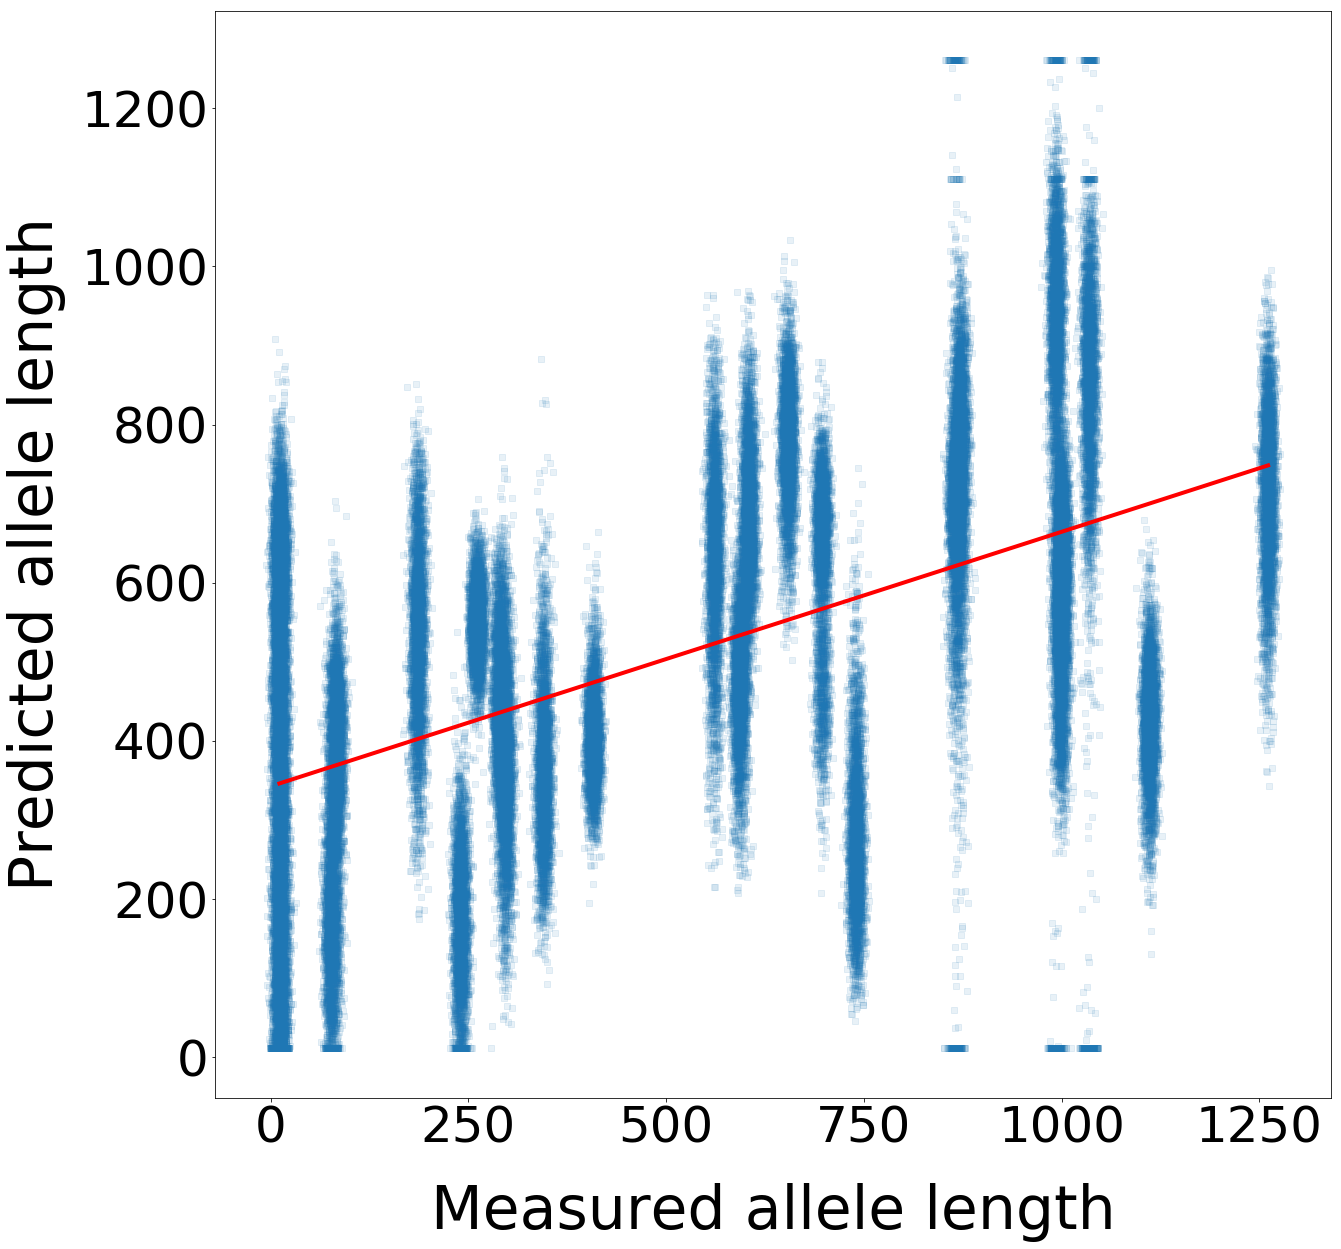
\includegraphics[width=\linewidth]{Nakamori_plot.png}
\caption{{\bf DM1-AS muscle MAL prediction.} 10,000 repetitions of cross-validated MAL prediction from genes labeled DM1-AS from muscle}
\label{fig1}
\end{figure}

\subsection*{Other models}

As described in \nameref{data_preparation}, we have used a model based on feature selection from sets of candidate mRNA biomarkers to predict the MAL of DM1 CTG repeat using PLSR. As reported in \nameref{PLSRPerformance}, the set of genes DM1-AS is the strongest predictor if we limit our consideration to predictors chosen a-priori, {\it i.e.} excluding TNNI1.

A potential source of criticism could be that the effect observed is a technical effect due to the choice or the implementation of the mathematical model used (PLSR). We thus re-ran the analysis as described before in \nameref{data_preparation} using three mathematically distinct models: lasso, random forest regression and linear regression.

We report the performance of these models in Table \ref{model_comparison}:

\begin{table}[!ht]
\begin{adjustwidth}{-2.25in}{0in} % Comment out/remove adjustwidth environment if table fits in text column.
\centering
\caption{{\bf 10000 repetitions of a simulation predicting MAL from muscle, using DM1-AS as a predicting set and a selection of mathematical models}}

\begin{tabular}{|l|l|l|l|l|}
\hline
 & PLSR & lasso & linear regression & random forest \\ \hline
R\textsuperscript{2} & 0.289 & 0.286 & 0.291 & 0.149 \\ \hline
p-value & 0.00434 & 0.00454 & 0.00418 & 0.0478 \\ \hline
\end{tabular}

\label{model_comparison}
\end{adjustwidth}
\end{table}

It should be noted that all models pick up statistically significant signal with both PLSR, lasso and linear regression performing almost equally well, and random forest performing about two times poorer (but still significantly better than a random predictor), which allows us to conclude that the effect observed is unlikely to be a modelling artifact.

%What may initially seem surprising, we can also obtain a good predictor without the need to pre-select genes. In fact if we train our model on all genes we still manage to detect good signal. While counter-intuitive, this finding is supported by related work of building complex feature predictors from SNP data ( reference Stephen Hsu's paper).

\subsection*{Applying the model in a clinical setting}

Let us now consider the potential application of this predictive model in the context of evaluating efficacy of a DM1 treatment. DM1 patients would undergo muscle biopsy before starting the treatment, and another biopsy after the treatment had been started and necessary biological changes to reverse DM1 symptoms had occurred. Both biopsies would be mRNA profiled, and the resulting profiles would be used to perform MAL predictions. We expect that pre-treatment prediction would correspond to the actual MAL of any given patient. We expect that post-treatment prediction of MAL would correspond to an ``effective MAL'', which we'd expect to be lower than the ``actual MAL'' in affected participants, as long as the treatment is effective and DM1-induced disruption of AS or APA, as measured by DM1-AS or DM1-APA biomarkers is measurably reversed in obtained mRNA profiles. Pre-treatment and post-treatment predictions could be combined into a statistic that, given enough patients, would allow us to quantify the efficacy of the treatment at the molecular level. We discuss this idea further in the chapter \nameref{poweranalysis}.

In some respects such a study could allow for better performance of the model, conceptually, it should be easier to capture DM1 specific expression changes in a setting where noise due to varied genetic backgrounds of participants can be reduced by looking at pairs of measurements of a single participant. There are a number of details in such study design, which need to be discussed by the community and decided upon, among others:
\begin{enumerate}
\item The mathematical basis of the model used. We propose a PLSR-based model, and demonstrate that models based on lasso and linear regression perform similarly, but other models can also be considered, in particular the work of Azencott {\it et al}. \cite{Azencott2013} in the context of L\textsubscript{1}-penalised regression (lasso) looks promising as it allows to incorporate prior biological knowledge, in the form of protein-protein interaction networks or other types of graph ontology, into the model, through the introduction of additional penalties based on discrete Laplacian, or apply alternative modelling strategies based on network flow, thereby increasing its predictive power.
\item The training/testing pre-treatment/post-treatment data split and which genes should be included in the model input.
\item The size of the study. Predictions in our study are based on 24 participants for blood and 18 for muscle. How much would the models' predictive power improve with a larger dataset?
\item Establishing the clinically relevant effect size. Pandey {
it et al.} \cite{Pandey2015} report various efficacies of a candidate DM1 treatment ISIS 486718 to lower toxic {\it DMPK} concentrations in wild-type and transgenic animal models and a range of tissues, starting with the efficacy of about 50\% in cardiac muscle, through about 70\% in skeletal muscle, up to about 90\% in liver and skeletal muscle. However, measuring DMPK levels may not necessarily directly correspond to the efficacy of treatment to reverse symptoms, and we could expect the rate of symptom reduction to be lower than the reported 50\% to 90\%. A difficult open question is what minimum treatment efficacy we are willing to accept as clinically significant.
\end{enumerate}

\subsection*{Power Analysis}

\label{poweranalysis}

Our final contribution, which is of critical significance in the context of any future clinical trial is a power analysis of the current model. We report power for a selection of possible treatment effect sizes (10\%, 20\% and 50\% reduction in effective MAL on a per-patient basis) and a selection of study participants. Our power is defined as ($1 - \beta$), where $\beta$ is a supremum of the probability of committing a type II error, with the supremum of the probability of committing type I error ($\alpha$) kept at a constant 0.05. Table \ref{power_table} reports power, ($1 - \beta$), to detect treatment effect of a two-tailed test with p-value cut-off of 0.05 (0.025 per tail), with the statistic simulated from MAL predictions of our model, for varying treatment effect and study sizes. We try to keep our cohort sizes realistic for a rare disease, {\it i.e.} we allow for patient numbers to range from 10 to 200.

Ideally we would like to be able to achieve power of more than 95\%, even with small treatment effect sizes and a small number of patients, but our model, trained on 18 participants, doesn't allow for such level of control over type II error for all but medium or large treatment effects (more than 20\% and 50\% respectively) and large (more than 140 participants) or medium-sized (more than 30 participants) clinical trials respectively.

However, our results combined with expected improvements of the model performance due to larger training samples, and better gene selections, such levels might be reached for medium treatment effect size (20\% reduction in effective MAL) and large clinical sizes.


\begin{table}[!ht]
\begin{adjustwidth}{-2.25in}{0in} % Comment out/remove adjustwidth environment if table fits in text column.
\centering
\caption{{\bf 10000 repetitions of a simulation predicting MAL from muscle cross-validated with a testing set separate from the training set.}}

\begin{tabular}{|l|l|l|l|}
\hline
study size (participants) & treatment effect 10\% & treatment effect 20\% & treatment effect 50\%  \\ \hline
10 & 0.100 & 0.209 & 0.635 \\ \hline
20 & 0.131 & 0.322 & 0.855 \\ \hline
30 & 0.162 & 0.423 & 0.947 \\ \hline
40 & 0.193 & 0.517 & {\bf 0.981} \\ \hline
50 & 0.226 & 0.596 & {\bf 0.994} \\ \hline
60 & 0.259 & 0.671 & {\bf 0.998} \\ \hline 
70 & 0.283 & 0.723 & {\bf 0.99908} \\ \hline
80 & 0.311 & 0.772 & {\bf 0.99979} \\ \hline
90 & 0.339 & 0.816 & {\bf 0.99998} \\ \hline
100 & 0.370 & 0.851 & {\bf 0.99998} \\ \hline
110 & 0.39592 & 0.88058 & {\bf 0.99999} \\ \hline
120 & 0.41811 & 0.90148 & {\bf 1.0} \\ \hline
130 & 0.44787 & 0.92379 & {\bf 1.0} \\ \hline
140 & 0.46685 & 0.93737 & {\bf 1.0} \\ \hline
150 & 0.49964 & {\bf 0.95245} & {\bf 1.0} \\ \hline
160 & 0.52316 & {\bf 0.96216} & {\bf 1.0} \\ \hline
170 & 0.54467 & {\bf 0.96901} & {\bf 1.0} \\ \hline
180 & 0.56775 & {\bf 0.97662} & {\bf 1.0} \\ \hline
190 & 0.58901 & {\bf 0.9809} & {\bf 1.0} \\ \hline
200 & 0.61316 & {\bf 0.9859} & {\bf 1.0} \\ \hline
\end{tabular}

\label{power_table}
\end{adjustwidth}
\end{table}

\subsection*{Limitations} \label{limitations}
A source of potential criticism is that muscles of DM1 patients have physiological differences (atrophy, increased fat content), especially when disease is severe. Quite possibly observed changes in AS/APA are partly attributable to these physiological differences in DM1 as opposed to purely biomolecular differences. The structure of this counter-argument could be as follows:

Muscles of DM1 patients have higher fat content than affected controls.
Muscle samples collected from DM1 patients have higher ratio of intermuscular adipocytes to myocytes.
Adipocytes have different AS/APA profiles than myocytes.
Observed AS/APA changes in the DM1 spectrum are mostly derived from differences in adipocyte/myocyte profile.
As a result, mRNA study of muscle tissue is no more effective (and possibly less effective) than a blinded study based on pathophysiological inspection of the tissue.

This argument can, of course be extended to other physiological changes than increased fat content, and other molecular events than AS/APA. Bachiński for example proposes that splicing changes could be a secondary result of muscle regeneration \cite{Bachinski2014}.
There are multiple ways to address these concerns:

\begin{enumerate}
\item Alternative designs based on tissue culture models, where in-vivo limitations are reduced, with homogeneity of the cellular composition of the model being a big advantage.
%\item Alternative designs based on single-cell next-gen sequencing.
\item Investigating methods to correct for potential ``physiological'' covariates ({\it e.g.} fat content), using purely statistical techniques to estimate covariate influence from gathered data and existing prior information ({\it e.g.} mRNA profiles of adipocytes), or biological methods, such as a very recent effort to collect higher quality muscle samples through MRI-guided biopsy \cite{Saskie2018}.
\item Discovering DM1 biomarkers in blood, as opposed to muscle. Blood, being much more homogeneous tissue than muscle is expected to be less prone to the existence of confounding variables. Additionally, necessity of muscle sampling was highlighted to be a ``main drawback'' \cite{Nakamori2013}. However, achieving this would require at least two separate, successful studies, one to identify biomarkers and one to evaluate them. Even if blood biomarkers were identified, their clinical utility might be limited, as a reduction of an effective MAL in blood would not be as direct evidence of treatment effectiveness as such reduction in muscle.
\end{enumerate}


% Place tables after the first paragraph in which they are cited.
%\begin{table}[!ht]
%\begin{adjustwidth}{-2.25in}{0in} % Comment out/remove adjustwidth environment if table fits in text column.
%\centering
%\caption{
%{\bf Table caption Nulla mi mi, venenatis sed ipsum varius, volutpat euismod diam.}}
%\begin{tabular}{|l+l|l|l|l|l|l|l|}
%\hline
%\multicolumn{4}{|l|}{\bf Heading1} & \multicolumn{4}{|l|}{\bf Heading2}\\ \thickhline
%$cell1 row1$ & cell2 row 1 & cell3 row 1 & cell4 row 1 & cell5 row 1 & cell6 row 1 & cell7 row 1 & cell8 row 1\\ \hline
%$cell1 row2$ & cell2 row 2 & cell3 row 2 & cell4 row 2 & cell5 row 2 & cell6 row 2 & cell7 row 2 & cell8 row 2\\ \hline
%$cell1 row3$ & cell2 row 3 & cell3 row 3 & cell4 row 3 & cell5 row 3 & cell6 row 3 & cell7 row 3 & cell8 row 3\\ \hline
%\end{tabular}
%\begin{flushleft} Table notes Phasellus venenatis, tortor nec vestibulum mattis, massa tortor interdum felis, nec %pellentesque metus tortor nec nisl. Ut ornare mauris tellus, vel dapibus arcu suscipit sed.
%\end{flushleft}
%\label{table1}
%\end{adjustwidth}
%\end{table}

\section*{Conclusion}

In this study we design and build a model based on Partial Least Squares Regression, which can explain as much as 28.9\% of the variance in DM1 CTG trinucleotide expansion from mRNA splicing data. Such explainability is only obtained when the model is trained on expression data from genes previously identified by Nakamori {\it et al.} \cite{Nakamori2013} as having disrupted AS on data obtained from muscle samples. We show how such model could be used in a clinical setting in the context of emerging DM1 treatments, and report power analysis to detect treatment effect depending on size of the treatment effect, type 1 error ($\alpha$) and potential size of the clinical trial. 

\section*{Supporting information}

% Include only the SI item label in the paragraph heading. Use the \nameref{label} command to cite SI items in the text.
%\paragraph*{S1 Fig.}
%\label{S1_Fig}
%{\bf Bold the title sentence.} Add descriptive text after the title of the item (optional).

%\paragraph*{S2 Fig.}
%\label{S2_Fig}
%{\bf Lorem ipsum.} Maecenas convallis mauris sit amet sem ultrices gravida. Etiam eget sapien nibh. Sed ac ipsum eget enim egestas ullamcorper nec euismod ligula. Curabitur fringilla pulvinar lectus consectetur pellentesque.

%\paragraph*{S1 File.}
%\label{S1_File}
%{\bf Lorem ipsum.}  Maecenas convallis mauris sit amet sem ultrices gravida. Etiam eget sapien nibh. Sed ac ipsum eget enim egestas ullamcorper nec euismod ligula. Curabitur fringilla pulvinar lectus consectetur pellentesque.

%\paragraph*{S1 Video.}
%\label{S1_Video}
%{\bf Lorem ipsum.}  Maecenas convallis mauris sit amet sem ultrices gravida. Etiam eget sapien nibh. Sed ac ipsum eget enim egestas ullamcorper nec euismod ligula. Curabitur fringilla pulvinar lectus consectetur pellentesque.

\paragraph*{S1 Appendix.}
\label{AppendixA}
{\bf Code \& how to run it.} All of the computer programs written for this study can be \hyperlink{https://github.com/picrin/clinical_applications}{found on github}.

The following instructions should allow one to independently verify results of our simulations (also available in the repository).

We advise that all of this code be run on a machine with 64 GB of RAM or more, given that some parts of the pipeline can use up in excess of 32 GB of RAM. We were able to successfully execute the entire analysis using an AWS ``m5.4xlarge'' EC2 instance. We found the default amount of storage, 8 GB, to be insufficient to store both the primary data and intermediate computations. We increased the amount of storage to 100 GB. We remove all networking restrictions on the instance, to allow for remote access of jupyter notebooks, which contain our pipeline.

We had to apply the following shell commands to set up the machine:


\begin{enumerate}

\item sudo apt-get update
\item sudo apt-get upgrade
\item sudo apt-get install python3-pip
\item git clone https://github.com/picrin/clinical\_applications.git
\item pip3 install jupyter

\end{enumerate}

All data and metadata used in this study are available in publicly accessible s3 bucket, with the following paths: ``dm1-biomarkers/CEL'', ``dm1-biomarkers/annotations'' respectively. These datasets need to be copied to the root of the ``clinical\_applications'' repository as directories ``CEL'' and ``annotations'' respectively.

All required third-party dependencies can be installed from the provided ``requirements.txt''

Finally, ``jupyter notebook --ip 0.0.0.0 --port 8888'' can be issued to start the notebook server, which we can access remotely, using a DNS entry allocated for our EC2 instance and provided that communications on our chosen port is configured to be accessible through the AWS firewall.

We now run notebooks in the following order:

\begin{enumerate}

\item ``parse\_chip\_data.ipynb''. This part of the pipeline is responsible for determining probeset ids, sequences of probes and probe coordinates on the chip. It produces an intermediate file with data adhering to the following schema: ``probeset, x, y, sequence''.
\item ``parse\_csv\_annotations.ipynb''. Here, we determine ``genomic'' metadata, i.e. chromosomomal coordinates and strandedness.
\item ``unpack\_CEL\_files.ipynb''. Here we use our own contribution to Biopython to parse the binary CEL v4 file format, which is what all our microarray data uses.
\item ``quantile\_normalise.ipynb''. Here we perform quantile normalisation of our microarray data.
\item ``reannotate\_probeset\_level.ipynb''. Here we verify Affymetrix's annotation. We determine that over 1\% probes are incorrectly annotated. We discard these probes. We limit our attention to probes, which belong to chromosomes chr1-chr22, X, Y and the mitochondrial DNA (M).
\item ``intervaltrees.ipynb''. Here we carry out an exclusive filtering, choosing probes, which are identified by ``gencode.v26lift37.annotation.gtf'' as having ``transcript\_type'' equal to ``protein\_coding'',  or ``gene\_type'' equal to  ``protein\_coding'', as well as the exon type equal to ``CDS'' (Coding sequence) or ``UTR'' (5' or 3' untranslated regions).
\item ``merge\_annotation\_experiment.ipynb''. Here we produce a single file per human gene, as identified in GENCODE v26, with data from all participants for all probes for that gene.
\item ``predictions.ipynb''. Here we run our PLSR model to predict MAL from the microarray data.
\item ``power\_analysis.ipynb''. Here we run power analysis presented in \nameref{ResultsDiscussion}.

\end{enumerate}

\paragraph*{S2 Appendix.}
\label{Appendix3}
{\bf DM1-AS}

DTNA FHOD1 RYR1 MBNL1 MBNL2 ARFGAP2 TBC1D15 GFPT1 NFIX CAPZB CAPN3 UBE2D3 USP25 VPS39 SOS1 ANK2 LDB3 BIN1 TXNL4A CACNA1S DMD OPA1 ATP2A1 IMPDH2 NRAP ABLIM2 PDLIM3 ATP2A2 VEGFA TTN MLF1 ALPK3 KIF13A CLCN1 PHKA1 COPZ2 INSR CAMK2B


\paragraph*{S3 Appendix.}
\label{Appendix2}
{\bf DM1-APA}

ABCA1 MEF2C PDLIM5 KIF1B CHRNA1 KCNK7 MDN1 SPATS2L TPM3 ILF3 MBNL2 SLC25A36 CLDND1 DES TPM1 OSBPL1A TPM2 HDAC11 AP1G1 CELF1 FASTK LDB3 NDUFB10 NR2F1 PCMT1 PCM1 DAPK2 RTN2 RIN1 MORC3 PLIN2 BRSK2 CIRBP TJP2 TTYH3 PIK3C2B PFKFB2 PEBP4 ARHGEF7 DST KRBA1 MEF2D MGP GPS1 MTCH1 SNX1 NUP43 TMEM38B SAMD4A EZR TBL2 SMIM3 CDC42 MYH6 MEF2B IDH3A CEBPA CACNA1G ALG3 SPEG DNAJB6 SPTB AMHR2 AGL ASPH TNNI1 DVL3 ATP5E PDLIM2 BRWD1 CACNB1 LMNA COPS4 KDELR1 SETD3 LAMP2 PCBD2 TGFBI U2SURP RAB24


%\paragraph*{S1 Table.}
%\label{S1_Table}
%{\bf Lorem ipsum.} Maecenas convallis mauris sit amet sem ultrices gravida. Etiam eget sapien nibh. Sed ac ipsum eget enim egestas ullamcorper nec euismod ligula. Curabitur fringilla pulvinar lectus consectetur pellentesque.

\section*{Acknowledgments}
We would like to thank the Marigold foundation for organising and funding DMBDI.

Adam Kurkiewicz would like to thank the college of Medical, Veterinary and Life Sciences as well as the Engineering and Physical Science Research Council for financing his Doctoral Training Programme stipend, student fees and his research fund.

\nolinenumbers

% Either type in your references using
% \begin{thebibliography}{}
% \bibitem{}
% Text
% \end{thebibliography}
%
% or
%
% Compile your BiBTeX database using our plos2015.bst
% style file and paste the contents of your .bbl file
% here. See http://journals.plos.org/plosone/s/latex for 
% step-by-step instructions.
% 

\bibliography{thebibliography}

%\begin{thebibliography}{10}

%\end{thebibliography}
\end{document}
